\subsection{UC2 - Salvataggio magazzino}
\begin{figure}[H]
  \centering
  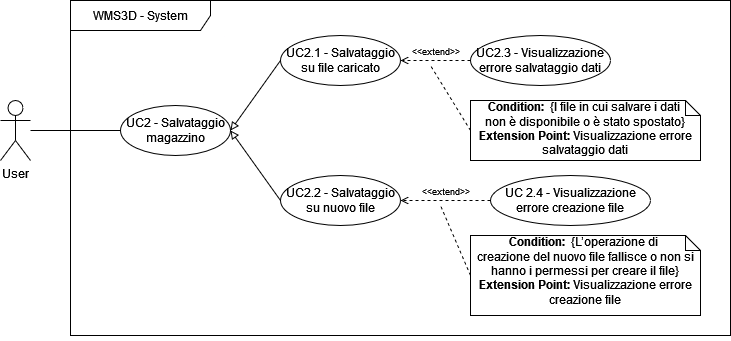
\includegraphics[width=0.8\textwidth]{UC_diagrams_1-10/UC2_sys.drawio.png}
   \caption{Diagramma UML UC2 - Salvataggio magazzino}
\end{figure}
\begin{itemize}
    \item \textbf{Attori:} User.
    \item \textbf{Pre-condizione:}  L'utente ha creato un magazzino [UC1] e lo sta visualizzando [UC3].
    \item \textbf{Post-condizione:} L'utente salva su un file locale i dati aggiornati di costruzione del magazzino.
    \item \textbf{Scenario Principale:} L'utente decide di salvare la planimetria 3D del magazzino e sceglie una modalità di salvataggio o su file già caricato al momento della creazione [UC2.1] o su un nuovo file [UC2.2]. I dati vengono poi salvati correttamente dall'utente nel file specificato.
    \item \textbf{Generalizzazioni:} Sono presenti due generalizzazioni:
    \begin{itemize}
        \item UC2.1 - Salvataggio su file caricato;
        \item UC2.2 - Salvataggio su nuovo file.
    \end{itemize}
    \item \textbf{Estensioni:} -
\end{itemize}


\subsubsection{UC2.1 - Salvataggio su file caricato}
\begin{itemize}
    \item \textbf{Attori:} User.
    \item \textbf{Pre-condizione:} L'utente ha creato un magazzino attraverso caricamento da file [UC1.1] e lo sta visualizzando [UC3].
    \item \textbf{Post-condizione:} L'utente salva sul file locale caricato in precedenza i dati aggiornati di costruzione del magazzino.
    \item \textbf{Scenario Principale:} L'utente decide di salvare la planimetria 3D su file già caricato al momento della creazione [UC1.1]. I dati vengono poi salvati correttamente dall'utente nel file specificato.
    \item \textbf{Generalizzazioni:} -
    \item \textbf{Estensioni:} È presente una estensione:
    \begin{itemize}
        \item UC2.3 - Visualizzazione errore salvataggio dati.
    \end{itemize}
\end{itemize}


\subsubsection{UC2.2 - Salvataggio su nuovo file}
\begin{figure}[H]
  \centering
  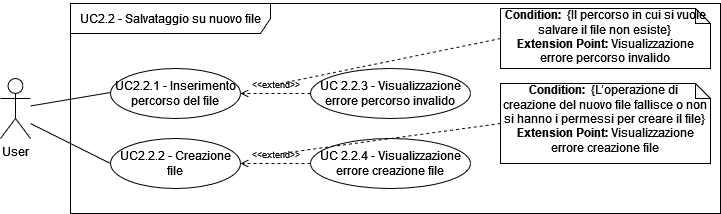
\includegraphics[width=0.8\textwidth]{UC_diagrams_1-10/UC2.2.drawio.png}
   \caption{Diagramma UML UC2.2 - Salvataggio su nuovo file}
\end{figure}
\begin{itemize}
    \item \textbf{Attori:} User.
    \item \textbf{Pre-condizione:} L'utente ha creato un magazzino [UC1] e lo sta visualizzando [UC3].
    \item \textbf{Post-condizione:} Il sistema crea un nuovo file con i dati di costruzione del magazzino.
    \item \textbf{Scenario Principale:} L'utente decide di salvare la planimetria 3D su un nuovo file. Quindi decide in che cartella locale memorizzare il nuovo file [UC2.2.1]. Il sistema poi creerà quest'ultimo con i dati della planimetria nella cartella specificata.
    \item \textbf{Generalizzazioni:} -
    \item \textbf{Estensioni:} È presente una estensione:
    \begin{itemize}
        \item UC2.4 - Visualizzazione errore creazione file.
    \end{itemize}
\end{itemize}


\paragraph{UC2.2.1 - Inserimento percorso del file}
\begin{itemize}
    \item \textbf{Attori:} User.
    \item \textbf{Pre-condizione:} L'utente vuole salvare i dati di costruzione del magazzino in un nuovo file.
    \item \textbf{Post-condizione:} L'utente specifica il percorso in cui salvare il file. Il sistema creerà il file in quella cartella.
    \item \textbf{Scenario Principale:} L'utente decide di salvare la planimetria 3D su un nuovo file. Quindi seleziona la cartella locale in cui memorizzare il file.
    \item \textbf{Generalizzazioni:} -
    \item \textbf{Estensioni:} È presente una estensione:
    \begin{itemize}
        \item UC2.2.2 - Visualizzazione errore percorso invalido.
    \end{itemize}
\end{itemize}

\paragraph{UC2.2.2 - Visualizzazione errore percorso invalido}
\begin{itemize}
    \item \textbf{Attori:} User.
    \item \textbf{Pre-condizione:} Il percorso in cui l'utente vuole salvare il file non esiste.
    \item \textbf{Post-condizione:} L'utente visualizza un messaggio d'errore e il salvataggio fallisce.
    \item \textbf{Scenario Principale:} L'utente visualizza un messaggio informativo sull'errore e ne conferma la ricezione. L'operazione, di conseguenza, fallisce.
    \item \textbf{Generalizzazioni:} -
    \item \textbf{Estensioni:} -
\end{itemize}

\subsubsection{UC2.3 - Visualizzazione errore salvataggio dati}
\begin{itemize}
    \item \textbf{Attori:} User.
    \item \textbf{Pre-condizione:}  Il file in cui salvare i dati non è disponibile o è stato spostato. 
    \item \textbf{Post-condizione:} L'utente visualizza un messaggio d'errore e il salvataggio fallisce.
    \item \textbf{Scenario Principale:}  L'utente visualizza un messaggio informativo sull'errore e ne conferma la ricezione. L'operazione, di conseguenza, fallisce.
    \item \textbf{Generalizzazioni:} -
    \item \textbf{Estensioni:} -
\end{itemize}


\subsubsection{UC2.4 - Visualizzazione errore creazione file}
\begin{itemize}
    \item \textbf{Attori:} User.
    \item \textbf{Pre-condizione:} L'operazione di creazione del nuovo file fallisce oppure non si hanno i permessi per creare il file.
    \item \textbf{Post-condizione:} L'utente visualizza un messaggio d'errore e il salvataggio fallisce.
    \item \textbf{Scenario Principale:} L'utente visualizza un messaggio informativo sull'errore e ne conferma la ricezione. L'operazione, di conseguenza, fallisce.
    \item \textbf{Generalizzazioni:} -
    \item \textbf{Estensioni:} -
\end{itemize}